\section{Discussion}\label{sec:discussion}

The separation of pipeline steps and their individual resource allocation allows for a more efficient usage of the \ac{HPC} cluster. Previously unnecessarily reserved threads and memory can now be used to process more samples in parallel. More resources can be utilized in parallel, as shown in \cref{subsection:resourceoptimization} and visualized side-by-side in \cref{figure:pipeline_benchmark_CPU_compared} and \cref{figure:pipeline_benchmark_memory_compared}.

\begin{figure}[H]
    \centering
	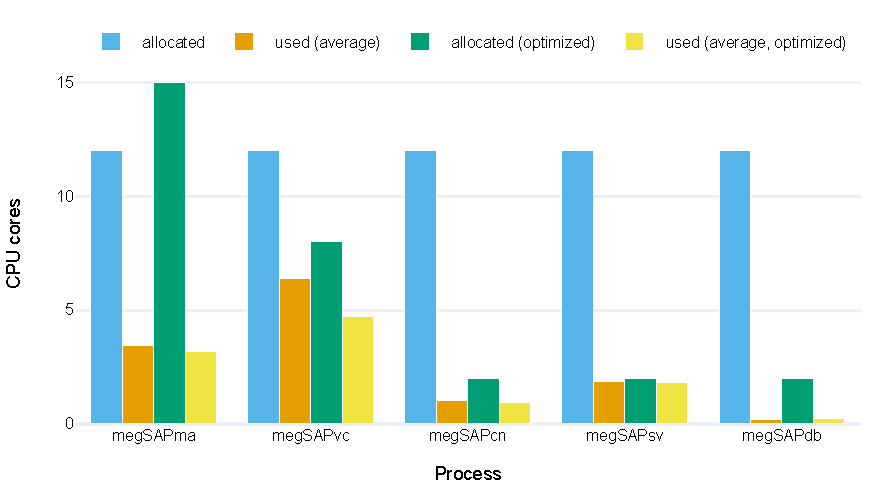
\includegraphics[width=\linewidth,height=\textheight,keepaspectratio]{pipeline_benchmark_CPU_compared}
	\caption{Average CPU usage of the Nextflow workflows compared}
	\label{figure:pipeline_benchmark_CPU_compared}
\end{figure}

\begin{figure}[H]
    \centering
	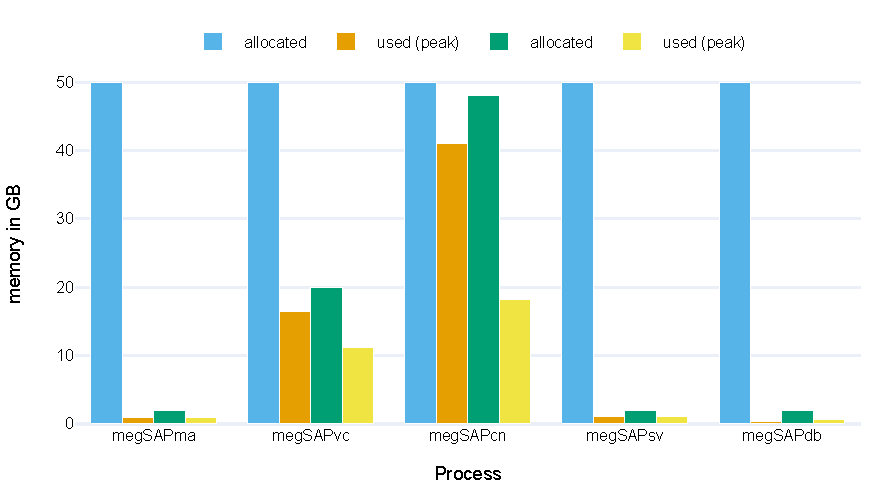
\includegraphics[width=\linewidth,height=\textheight,keepaspectratio]{pipeline_benchmark_memory_compared}
	\caption{Peak memory usage of the Nextflow workflows compared}
	\label{figure:pipeline_benchmark_memory_compared}
\end{figure}

To quantify the gains, the measuring unit \textit{CPU hours} respectively \textit{memory hours} is calculated for the reserved resources. As seen in \cref{equation:initialcpu,equation:initialmemory}, this resolves to \SI{138.0}{CPU~\hour} and \SI{575}{\giga\byte~\hour} for the initial workflow described in \cref{subsection:initialworkflow}.
\begin{equation}\label{equation:initialcpu}
    \begin{aligned}
        \SI{12}{CPU}\times\SI{11.5}{\hour} &= \SI{138.0}{CPU~\hour}
    \end{aligned}
\end{equation}
\begin{equation}\label{equation:initialmemory}
    \begin{aligned}
        \SI{50}{\giga\byte}\times\SI{11.5}{\hour} &= \SI{575}{\giga\byte~\hour}
    \end{aligned}
\end{equation}

After optimization, the result is \SI{79.563}{CPU~\hour} for reserved CPU resources and \SI{374.501}{\giga\byte~\hour} for memory as calculated in \cref{equation:optimizedcpu,equation:optimizedmemory} 
\begin{equation}\label{equation:optimizedcpu}
    \begin{aligned}
        \text{megSAPma: }\SI{15}{CPU}\times\SI{2.683}{\hour} &= \SI{40.245}{CPU~\hour}\\
        \text{megSAPvc: }\SI{8}{CPU}\times\SI{2.938}{\hour} &= \SI{23.504}{CPU~\hour}\\
        \text{megSAPcn: }\SI{2}{CPU}\times\SI{6.383}{\hour} &= \SI{12.766}{CPU~\hour}\\
        \text{megSAPsv: }\SI{2}{CPU}\times\SI{1.467}{\hour} &= \SI{2.934}{CPU~\hour}\\
        \text{megSAPdb: }\SI{2}{CPU}\times\SI{0.057}{\hour} &= \SI{0.114}{CPU~\hour}\\
        \hline
        \text{Optimized workflow } &= \SI{79.563}{CPU~\hour}
    \end{aligned}
\end{equation}
\begin{equation}\label{equation:optimizedmemory}
    \begin{aligned}
        \text{megSAPma: }\SI{2}{\giga\byte}\times\SI{2.683}{\hour} &= \SI{5.366}{\giga\byte~\hour}\\
        \text{megSAPvc: }\SI{20}{\giga\byte}\times\SI{2.938}{\hour} &= \SI{59.76}{\giga\byte~\hour}\\
        \text{megSAPcn: }\SI{48}{\giga\byte}\times\SI{6.383}{\hour} &= \SI{306.384}{\giga\byte~\hour}\\
        \text{megSAPsv: }\SI{2}{\giga\byte}\times\SI{1.467}{\hour} &= \SI{2.934}{\giga\byte~\hour}\\
        \text{megSAPdb: }\SI{1}{\giga\byte}\times\SI{0.057}{\hour} &= \SI{0.057}{\giga\byte~\hour}\\
        \hline
        \text{Optimized workflow } &= \SI{374.501}{\giga\byte~\hour}
    \end{aligned}
\end{equation}
This means that CPU resources are used \SI{42.35}{\percent} more efficient than before and memory is used \SI{34.87}{\percent} more economically after the optimizations as also shown in \cref{figure:pipeline_benchmark_efficiency}. 

A comparison of initial and optimized CPU and memory allocation over time is shown in \cref{figure:pipeline_cpu_compared_aoc,figure:pipeline_memory_compared_aoc}

\begin{figure}[H]
    \centering
	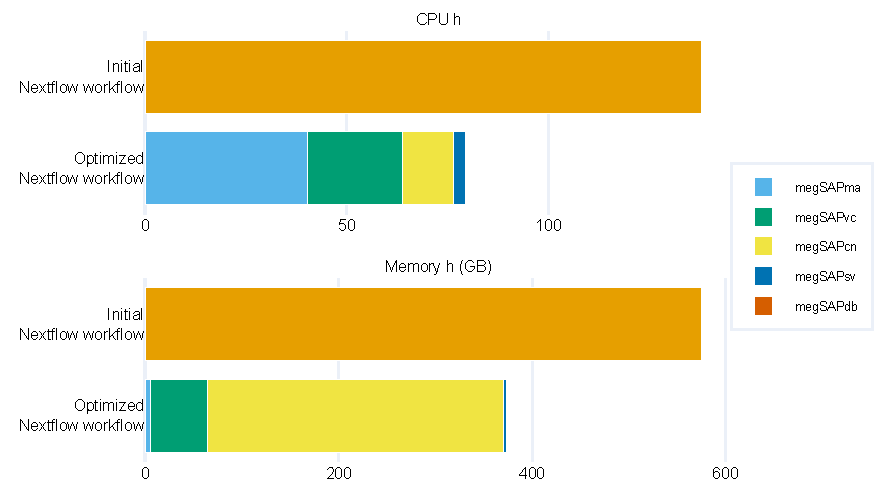
\includegraphics[width=\linewidth,height=\textheight,keepaspectratio]{pipeline_benchmark_efficiency}
	\caption{Efficiency after pipeline optimization}{Resource consumption of the megSAPdb process is too low to be rendered.}
	\label{figure:pipeline_benchmark_efficiency}
\end{figure}

\begin{figure}[H]
    \centering
	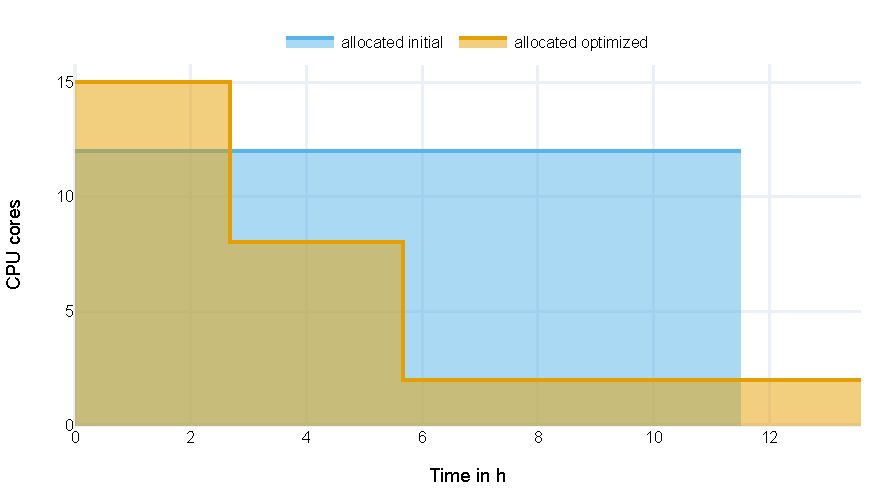
\includegraphics[width=\linewidth,height=\textheight,keepaspectratio]{pipeline_benchmark_CPU_compared_aoc}
	\caption{CPU allocation of initial and optimized workflows over time}
	\label{figure:pipeline_cpu_compared_aoc}
\end{figure}

\begin{figure}[H]
    \centering
	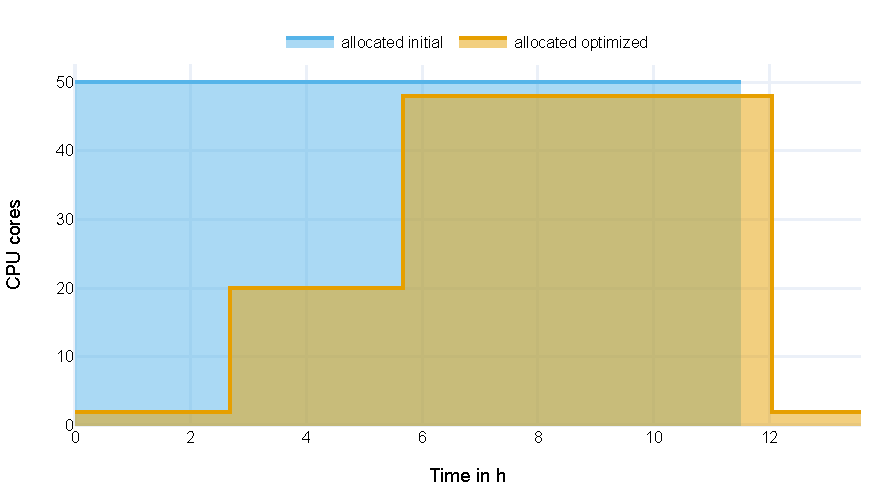
\includegraphics[width=\linewidth,height=\textheight,keepaspectratio]{pipeline_benchmark_memory_compared_aoc}
	\caption{Memory allocation of initial and optimized workflows over time}
	\label{figure:pipeline_memory_compared_aoc}
\end{figure}

This can also be transferred to the estimated cost of using \textit{\ac{AWS}} to compute the pipeline in the cloud. With the optimized pipeline, this amounts to \SI{26.33}{\$} as shown in \cref{sec:awscostestimation}. Using a m5.4xlarge instance type to run the pipeline in its previous state (see \cref{subsection:initialworkflow}) for \SI{11.5}{\hour} would raise this to \SI{29.77}{\$} (see \cref{appendix:awspricecalculationunoptimized} for details), saving \SI{11.56}{\percent}. This amount is lower than the realizable retrenchments for the \ac{HPC} cluster, as \textit{\ac{AWS}} instance types do not exactly match to the required resources and the overhead produces more cost than necessary.

These resource adjustments should be monitored and improved upon in the future. Slight changes might show improvements on execution time or allow for less resources to be allocated to some steps. A first example might be the \textttx{megSAPcn} step. Its memory consumption seems to be affected by the number of threads, as it dropped more than half after reducing the number of available CPUs.

Two different approaches can be taken to optimize the resource usage: 
\begin{enumerate}
    \item Using resources to process a sample as fast as possible. This may be needed to answer a particular time critical diagnostic question.
    \item Using resources to process multiple samples simultaneously as efficient as possible. Routine diagnostic profits from an average optimal processing time calculated over multiple samples. 
\end{enumerate}
As resource usage and runtime do not correlate linearly, but probably follow more of a sigmoid curve, these two approaches differ. For this thesis, the latter approach has been taken, as its goal is to process numerous samples retroactively. But the \ac{DoHG@MHH} sometimes has different needs regarding the speed of diagnostics, e.g., for the \textit{Baby Lion} study (see \autocite{MedizinischeHochschuleHannover2022}), which employs rapid whole-genome sequencing as described by \citeauthor{Saunders2012} \autocite{Saunders2012}, the pipeline should run as fast as possible. Handling both approaches may be put into practice for the \textit{Nextflow} pipeline by using different configuration profiles (see \autocite[Config profiles]{SeqeraLabs2022e}) for different needs.

Since the CPU utilization is only calculated as a weighted average, thread allocation is an explorative task. Additionally, \textit{\ac{megSAP}} combines too many tools into one step to make informed decisions on thread usage. This is particularly visible in the mapping step, as outlined in \cref{subsection:seperationofsteps}: The resource-intensive task \textit{SeqPurge} is combined with the, at least from a cluster perspective, idling task that waits for the \textit{DRAGEN} mapping to be done. To facilitate more optimization in the future, \textit{\ac{megSAP}} has to be separated into more individual steps. At best, each tool has its own process in \textit{Nextflow} in the future \textemdash this would render all the current \textit{PHP} scripts of \textit{\ac{megSAP}} obsolete and move all logic to \textit{Nextflow} - a vision worth considering.

Otherwise, the memory utilization is measured by peak usage and the optimization for each step, as presented in \cref{subsection:resourceoptimization}, can approach this optimum. These optimizations would also benefit from a fragmentation of the \textit{\ac{megSAP}} steps, as changes could be more precise and not only accommodate for the extremum usage of a whole pipeline step, but for each tool used \textemdash in the same manner as the CPU usage optimizations.

One pertinent measurement was not included for this thesis: disk utilization. The \ac{HPC} cluster does not have tiered storage. All data resides on the same network attached storage. Therefore, no actions could have been derived by any findings. But as the operations performed by the pipeline are using large files to begin with, it might be a promising endeavor to employ faster scratch devices during the pipeline run.

The implementation of \textit{Nextflow} also introduces a remedy for previous problems:
\begin{description}
    \item[Resilience] By leveraging \textit{Nextflow}'s built-in \textttx{maxRetries} directive (see \cref{subsection:resilienceandmonitoring}) it is possible to cure not reproducible pipeline errors. By simply restarting the relevant step with more resources, these errors can be automatically fixed.
    
    Nevertheless, it might be expedient to check for certain error-codes to react accordingly. For example, an out-of-memory error could be fixed systematically instead of just blindly trying the failed step again with more resources.
    
    \item[Reporting] The email reporting features of \textit{Nextflow} are a first step towards better monitoring of the pipeline. This also applies to the detailed reports generated by each workflow run.
\end{description}

The created \textit{Nextflow} workflow is hosted on the \ac{MHH}'s internal \textit{GitLab} severs. Using \textit{Git} as a version control system allows for tracking changes made to the workflow over time, so it can easily be reverted to previous versions if needed. Hosting the workflows in \textit{GitLab} also provides a backup and helps to ensure that the workflow is not lost in case of any data loss. \textit{GitLab} also makes it easier to share the workflow and to reuse it in different projects.

Two issues outlined in \cref{subsection:problem} were not fixed by the initial introduction of \textit{Nextflow}: the workflow still has to be triggered by a shell command and no accessible monitoring is possible during the pipeline run. Both of these impediments might be fixable by harnessing the features offered by \textit{Nextflow Tower} (see \autocite{SeqeraLabs2022g}). It promises enhanced monitoring, logging, and observability for workflows and streamlined deployment of pipelines by providing a easy to use web-based interface. Incorporating \textit{Nextflow Tower} into the newly built \textit{Nextflow} workflow will be the next project at the \ac{DoHG@MHH}.
